\documentclass[a4paper, 10pt, twocolumn, twoside]{article}

\usepackage{ISARC}

\usepackage{lscape}
\usepackage{hologo}
\usepackage{multirow}

\begin{document}

 % Do not change the following line
\linespread{0.5}

\title{BIM-FM interoperability: integrating existing FM platforms with visualization of IFC models}

\author{Andressa Oliveira$^{1}$, José Granja$^1$, Pedro Machado$^2$, Ali Motamedi$^3$, and Miguel Azenha$^1$}

\affiliation{
$^1$University of Minho, ISISE, ARISE, Department of Civil Engineering, Portugal\\
$^2$Matosinhos City Council, Portugal\\
$^2$Université du Québec à Montreal, École de Technologie Supérieure, Canada
}

\email{
\href{mailto:soliveira.andressa@gmail.com}{soliveira.andressa@gmail.com}, 
\href{mailto:e.author1@aa.bb.edu}{Email Granja},
\href{mailto:e.author1@aa.bb.edu}{Email Pedro Machado},
\href{mailto:e.author1@aa.bb.edu}{Email Ali},
\href{mailto:e.author1@aa.bb.edu}{Email Miguel}
}


% Do not change the following three lines
\maketitle 
\thispagestyle{fancy} 
\pagestyle{fancy}



\begin{abstract}
The adoption of Building Information Modelling (BIM) in the operational phase of buildings is still restricted. One of the factors hindering adoption of the methodology is the lack of BIM capabilities in Facility Management (FM) platforms, such as three-dimensional visualisation of the buildings to be managed. This article presents a solution designed in collaboration with the Matosinhos City Council in Portugal to enable the management of its assets using the BIM methodology. The purpose of the solution is to integrate the current management platform used by the council (Infraspeak) with three-dimensional visualisation resources, and to allow the consultation and manipulation of operational data directly and integrated with this visualisation. The use of information models (BIM models) that follow the IFC (Industry Foundation Classes) scheme has been considered for asset visualisation. In this context, an integrated and customised web platform was developed using the IFCjs library to manipulate, investigate and visualise IFC files. In addition, the platform allows direct connection to the Infraspeak database via its Application Programming Interface (API). This article details the development process of the integration platform, its key components and its interoperability with Infraspeak. The solution developed is an innovative approach to the current limitations in operations management and supports the wider adoption of BIM for the FM area.
\end{abstract}

\begin{keywords}
Facility Management (FM); Building Information Modelling (BIM); Interoperability; Integration
\end{keywords}

% AS SESSÕES DO ARTIGO COMEÇAM AQUI

\section{Introduction}
\label{sec:Introduction}

The operational phase of a built asset represents the largest part of its life cycle, totalling approximately 60\% of the costs associated with it [1]. Facility Management (FM) is the discipline responsible for the functionality, comfort and safety of facilities in the built environment [2], and is one of the fastest growing sectors in the construction industry [3]. With the industrialisation of this sector [4], asset managers have become increasingly interested in implementing the BIM methodology to support operations management [3]. This integrated information management methodology can bring numerous advantages to a sector that has to deal with a large amount and variety of data from different sources [5]. Due to the variety and complexity of assets that public buildings and/or large buildings can present [3], the implementation of the BIM methodology can bring great benefits in supporting operations managers looking to improve the efficiency of FM processes in these types of buildings. Despite the various advantages found in the literature, there is still resistance to adopting BIM for asset operation [6], and managers are faced with a built heritage that is already in the operational phase but is not yet managed, for the most part, with the support of the BIM methodology.

The current scenario shows that the use of management platforms that assist in the operation of built assets, such as Computerized Maintenance Management System (CMMS), Computer Aided Facility Management (CAFM) and Intelligent Maintenance Management Platform (IMMP), is already widespread [4], [5]. However, current management models are not prepared for the rapid adoption of BIM because they are heavily based on traditional methods, such as the use of physical documents, even when computerised platforms are used [5]. For a wider and more efficient adoption of BIM in the operational sector, it is necessary to spread knowledge about the methodology's information management processes, following the guidelines of ISO 19650-3 [7], and thus adapting management models so that they can cope with emerging technologies [6]. This updating of the management model includes, in addition to processes, the use of platforms capable of integrating different databases, including information models [1]. In the BIM methodology, information models are the main source of information on an asset and can include, among other things, information blocks containing the three-dimensional geometric representation of the asset [8]. In this context, information models must be prepared in such a way as to be able to integrate with the management platforms used by operations managers. From this context emerges the need to support the implementation of the BIM methodology in operations management processes, with a focus on integration between different data sources. Studies in this area could have an impact on the adoption of BIM in the operational phase of assets, especially in the public sector.

From this scenario emerged a partnership between the Matosinhos City Council (CMMatosinhos), in Portugal, and the University of Minho (UMinho). The aim of this partnership is to support the management and operation of municipal assets by integrating the BIM methodology into the management platform already used by CMMatosinhos, Infraspeak. This platform is an IMMP and allows users to interact with a web interface to access its functionalities, but does not allow visualisation of the buildings and assets managed. The IMMP also allows access to its functionalities via an Application Programming Interface (API). Therefore, the ultimate goal of this work is to develop a web platform capable of integrating the IMMP database with the three-dimensional visualisation of the assets to be managed, allowing the consultation, editing and insertion of information associated with these assets. From the developments of this partnership, the management and operations area of CMMatosinhos will be able to add geometric information to the decision-making process (e.g. with the visual distribution of spaces/equipment in need of maintenance actions within a building, it will be possible to define more efficient action routes).

\emph{erro}

efficient). The integration platform to be developed needs to allow communication between two different databases: the IMMP database, which contains the information needed to operate the assets; and the block of information containing the geometry of the buildings and assets to be managed. For the sake of simplicity, the block of information with three-dimensional visualisation will be referred to as the model throughout this article.

The first stage in the development of this study (section 2) included defining the objectives of CMMatosinhos and the functionalities of the integration platform to be developed. After defining the functional requirements, it was possible to establish the interaction processes between the different databases (section 3.1) and define the information exchange requirements (EIR) to guide the development of the models that will be accessed from the developed platform (section 3.2). The EIR was developed in a simplified way and the methodology of the level of information required [9] was used to define the requirements. Subsequently, the integration platform was implemented, with tests carried out and the use of an example model (prototype) developed from the requirements defined previously (section 3.3). Finally, the conclusions and discussions relevant to the research carried out are summarised in section 4.

\section{Methodology and functional requirements for the platform}
\label{sec:methodology}

The partnership required the development of a platform capable of integrating the IMMP used by CMMatosinhos with the ability to visualize and manipulate three-dimensional models of buildings under its management. It also encompasses the definition of information requirements (EIR) for models to be used within this platform. Meetings with the town hall allowed a detailed understanding of its objectives with the platform, which were necessary to establish its foreseen functionalities. Initially, the platform should provide a building selection interface. The platform should support comprehensive 3D visualization options, including viewing the entire building, individual floors, or specific elements with open requests. Additionally, users should be able to interact with the 3D model by selecting assets directly from the 3D representation. The platform should display the building's identification details and the number of open requests linked to it. For asset-specific information, the platform should allow users to identify assets through selection and display the total number of open requests associated with a particular asset. Furthermore, it should include a feature to redirect manager users to the asset's IMMP dedicated page for more in-depth information. Lastly, the platform should allow users to submit requests associated with specific assets.

From the functionalities, it was established that the web platform would contain two pages: the building selection page and the interaction page. Regarding the users, it would include two different user profiles (manager and common user). Both user profiles would allow users to visualize the building, interact with its 3D representation, see identification information about the building and its assets, and submit requests related to assets (equipment or spaces). In addition, the manager user profile would be able to visualize information regarding the open requests related to the building, spaces, or assets and be redirected to specific pages of the IMMP. The development of the web platform can be divided into two layers: frontend and backend. HTML, CSS and JavaScript were used for the frontend. Among the platform's functionalities, those related to dealing with the IFC model were developed with the support of the IFCjs open-source library. This library allows the creation of customised and interactive viewers, including viewing the entire building or subsets of it and selecting specific elements within the model. In addition, the library allows you to access element properties and extract information from them. The backend was developed in Python using the Flask web framework. The prototype building model was developed on the Autodesk Revit 2023 platform and followed previously defined information requirements. This model was then exported following the IFC scheme (IFC4 ADD2 TC1) \cite{BuildingSMARTa}.

\section{Implementation}
\label{sec:implementation}

To develop this work, the "IMMP database" must be integrated into a web platform presenting the IFC model visualization. The integration is only possible if elements are uniquely identified and associated between the IMMP database and the IFC models (hosted in the "Models database"). Considering the functionalities to be implemented \ref{sec:methodology}, three types of elements are essential to the platform's objectives: \emph{locations}, \emph{equipment} and \emph{requests}. \emph{Locations} represent spatial assets or spaces that comprise the buildings and are essential to the equipment's localization. \emph{Equipment} is any physical asset from the CMMatosinhos' inventory (vehicles, chairs, ladders, etc.). Finally, \emph{requests} represent the solicitation for an operation action to be carried out and are always associated with the other types of elements (\emph{equipment} or \emph{location}). Figure \ref{fig_fluxo} shows the flow of information between the platform layers (frontend and backend) and how the manager user type interacts with the platform.

\begin{figure}[!htb]
    \centering
    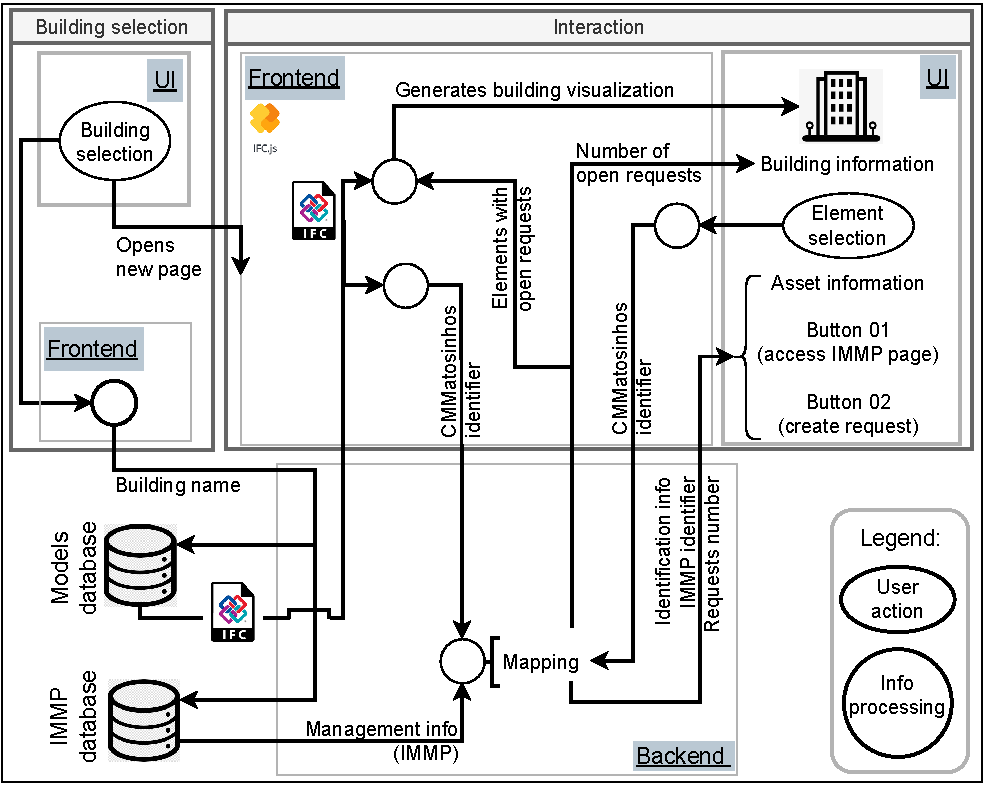
\includegraphics[width=0.48\textwidth]{Images/fluxo.pdf}
    \caption{Information flow on the web platform}
    \label{fig_fluxo}
\end{figure}

\subsection{Unique identifiers}
\label{subsec:identifiers}

To determine how the elements would be linked, it was necessary to understand how they are identified within the IMMP database (IMMP identifiers) and how CMMatosinhos recognizes them in its inventory (CMMatosinhos identifiers).

\paragraph{IMMP identifier}:

The IMMP database contains two categories of entries for \emph{locations}: LOCATION and ELEMENT. Within the LOCATION category, they are organized hierarchically and identified by a unique attribute called "local\_id". On the other hand, the ELEMENT category includes two types of assets: EQUIPMENT and LOCAL. In this context, the \emph{locations} classified as ELEMENT are specifically of the type LOCAL, representing the lowest level of the spatial hierarchy found in the LOCATION category. These represent individual spaces, such as rooms. Regarding the \emph{equipment}, those are entries of the ELEMENT category and EQUIPMENT type. The "element\_id" attribute uniquely identifies each element from the ELEMENT category. The code contained in these attributes ("local\_id" and "element\_id") is generated automatically by the IMMP, and does not correspond to the CMMatosinhos inventory. Therefore, the "local\_id" and "element\_id" attributes are considered to be the IMMP identifiers for \emph{locations} and \emph{equipment}, respectively.

The \emph{requests} elements are categorized as \emph{failure} within the IMMP database, and those designated as "open" are the relevant ones for this work since they still require actions. Since \emph{requests} are not physical assets, it was necessary to analyze their correlation with \emph{equipment} and \emph{location} elements, alongside the attributes of the \emph{failure} itself. Each request (\emph{failure}) is uniquely identified by the "failure\_id" attribute and includes a "local\_id" attribute that specifies the \emph{location} associated with the request. Contrarily, information regarding its connection to \emph{equipments} can only be accessed through the relationships of the \emph{equipment} elements, which allow visualization of the corresponding "failure\_id" codes.

\paragraph{CMMatosinhos identifier}:

"CMMatosinhos identifiers" relate to the code used by CMMatosinhos to identify its assets within its inventory. Currently, these codes are part of the information associated with the assets within the IMMP database. Therefore, the "CMMatosinhos identifiers" analysis was conducted using the IMMP database, focusing on attributes that provide information relevant to identifying assets from the CMMatosinhos perspective. Among the three elements (\emph{equipment}, \emph{location}, and \emph{requests}), \emph{requests} do not have a CMMatosinhos identifier as they do not represent physical assets, being not part of CMMatosinhos' inventory. 

As for \emph{locations}, the value of the "full\_code" attribute represents the nomenclature used by CMMatosinhos to identify spaces hierarchically, containing a unique code for each location. As for \emph{equipment}, the value of the "nfc\_code" attribute was selected as a potential unique identifier. However, not all equipment contains associated NFC codes, which implies that it could not be used as the identification key for this type of asset. In a second analysis, the "code" attribute was selected for this purpose. Within the CMMatosinhos inventory, the value of this attribute is filled in using coding specific to the type of equipment (chair, vehicle, etc.). However, the end user clarified that this coding might not be unique for some specific types of equipment but, if there were more than one \emph{equipment} element with the same code, those \emph{equipment} would not be in the same space.

Therefore, the combination of the attributes "code" of the active piece of equipment and "full\_code" of the location where it is located associated within the model, was defined as the CMMatosinhos identifier for the equipment. Finally, using the necessary level of information methodology (section 3.2), these identifiers were organised as properties that should be associated with the model elements. In Table 2, the term "Code" was used to represent these identifiers.

\subsection{Level of information need}
\label{subsec:loin}

ISO19650-3 [7], for asset operation, states that the development of the EIR should be derived from organizational (OIR) and operational (AIR) requirements. OIR and AIR were not developed for this work, and the objectives defined in Table 1 served as premises for the development of the simplified EIR.

In order to define the level of information required, it was considered that the model should allow visualisation of the building and assets to be managed, and contain only alphanumeric information relating to general asset information and that required for integration with the IMMP database (CMMatosinhos identifiers). As for the elements to be modelled (Table 2), three main groups of objects were defined: architecture, equipment and locations.

\begin{table*}[!htb]
    \renewcommand{\arraystretch}{2}
    \centering
    \caption{Level of information need for architectural elements, equipment and locations}
    \label{loin_equipment}
    \begin{tabular}{p{0.8cm}|p{3.7cm}|p{3.2cm}p{3.2cm}p{2.0cm}}
    \hline
    \multicolumn{2}{r}{\textbf{Objects:}} & \textbf{Archit. elements} & \textbf{Equipment} & \textbf{Locations}\\
    \hline
    \multicolumn{2}{r}{\textbf{IFC Class:}} & \textbf{Variable} & \textbf{Variable} & \textbf{IfcSpace}\\
    \hline
    \multicolumn{5}{l}{\textbf{Geometrical information}} \\
    \hline
    \multicolumn{2}{l}{Detail} & Real representation of external limits. Single element without layers or components. & Simplified outer shell, real volumes and dimensions. Single element without layers or components. & Real volume.\\
    \multicolumn{2}{l}{Dimensionality} & 3D & 3D & 3D\\
    \multicolumn{2}{l}{Location} & Relative & Relative & Relative\\
    \multicolumn{2}{l}{Appearance} & Colour must be similar to reality, without textures. & Colour must be similar to reality, without textures. & Not visible\\
    \hline
    \multicolumn{5}{l}{\textbf{Alphanumerical information}} \\
    \hline
    \multicolumn{5}{l}{Attributes} \\
    \hline
    & Attribute name & \multicolumn{3}{c}{Content}\\
    \hline
    & LongName & X & X & Name\\
    \hline
    \multicolumn{5}{l}{Properties} \\
    \hline
    Group & Property name & \multicolumn{3}{c}{Content}\\
    \hline
    \multirow{4}{*}{**} & Codigo\_CMMatosinhos & X & Code & X\\
    & Local\_CMMatosinhos & X & X & Code\\
    & Categoria\_CMMatosinhos & X & Category & X\\
    & Tipo\_CMMatosinhos & X & Category description & X\\
    \hline
   \multirow{6}{*}{\rotatebox{90}{\textbf{Legend}}} & \multicolumn{4}{l}{\textbf{Variable}}\\
    & \multicolumn{4}{l}{    IFC classes vary depending on the architectural element or equipment.}\\
    & \multicolumn{4}{l}{\textbf{**}}\\
    & \multicolumn{4}{l}{    Name fo group of properties: CMMatosinhos\_Identification}\\
    & \multicolumn{4}{l}{\textbf{X}}\\
    & \multicolumn{4}{l}{    Objects of this type must not contain this property or attribute.}\\
    \hline
    \end{tabular}
\end{table*}

In this case, the architecture would serve the purpose of visualisation and only the geometric information aspects of the necessary level of information were required for this group. Of the three types of elements analysed in the previous subsection, applications were excluded as their visualisation was not required. For premises and equipment, geometric and alphanumeric information requirements were defined. As for the building as a whole (Table 3), since its geometry was already covered by the previous objects, only alphanumeric information requirements were defined. Non-applicable aspects are not shown in the tables.

\begin{table*}[!htb]
    \renewcommand{\arraystretch}{2}
    \centering
    \caption{Level of information need for architectural elements, equipment and locations}
    \label{loin_equipment}
    \begin{tabular}{p{5.1cm}|p{4.3cm}|p{4.3cm}}
    \hline
    {\raggedright\textbf{Objects:}} & \multicolumn{2}{l}{\textbf{Building}}\\
    \hline
    {\raggedright\textbf{IFC Class:}} & \multicolumn{2}{l}{\textbf{IfcBuilding}}\\
    \hline
    \multicolumn{3}{l}{\textbf{Alphanumerical information}} \\
    \hline
    \multicolumn{3}{l}{Attributes} \\
    \hline
    & Attribute name & Content\\
    \hline
    & LongName & Name\\
    \hline
    \multicolumn{3}{l}{Properties} \\
    \hline
    Group & Property name & Content\\
    \hline
    CMMatosinhos\_Identification & Local\_CMMatosinhos & Code\\
    \hline
    \end{tabular}
\end{table*}

\subsection{Platform development}
\label{subsec:platform}

The development of the platform, the tests carried out and the meetings with the end user took place iteratively and the platform's capabilities were gradually expanded. During development, it was possible to identify the limitations of the IMMP API and improve the information exchange processes. One of the optimisations implemented was the mapping between all the objects in the model (equipment or sites) and their respective open requests (open failures) (visible in Figure 2 in the backend). This mapping has been programmed to occur automatically as soon as the building is selected, and generates a direct association between the unique identifiers of the elements ("element\_id" and "local\_id") and the associated "failures\_id". This mapping also includes information such as the degree of prioritisation and the status of the request (failure). The decision was made because this information needs to be quickly visualised by the user and updated when they move between selected elements, which ultimately improves the end-user experience.

Figure \ref{fig_plataforma} shows the visualisation of the integration platform accessible by the end user. The screenshot is of the management area, with visualisation enabled by floor and after selecting an element. The management area includes an upper section (Figure 4 a) with data relating to the building's identification and the possibility of editing the visualisation mode: whether by floor or entire building, whether all elements or only those with open requests. The next section (Figure 4 b) displays a warning about the presence and number of open requests associated with the building. The side menu (Figure 4 c) relates to asset information and is inserted into the user interface when a piece of equipment or location is selected. In this menu, it is possible to view information identifying the selected asset, the number of open requests associated with the asset, access the redirection to the asset's page within IMMP and the creation of orders associated directly with the asset, which are automatically registered within the IMMP platform.

\begin{figure*}[!htb]
    \centering
    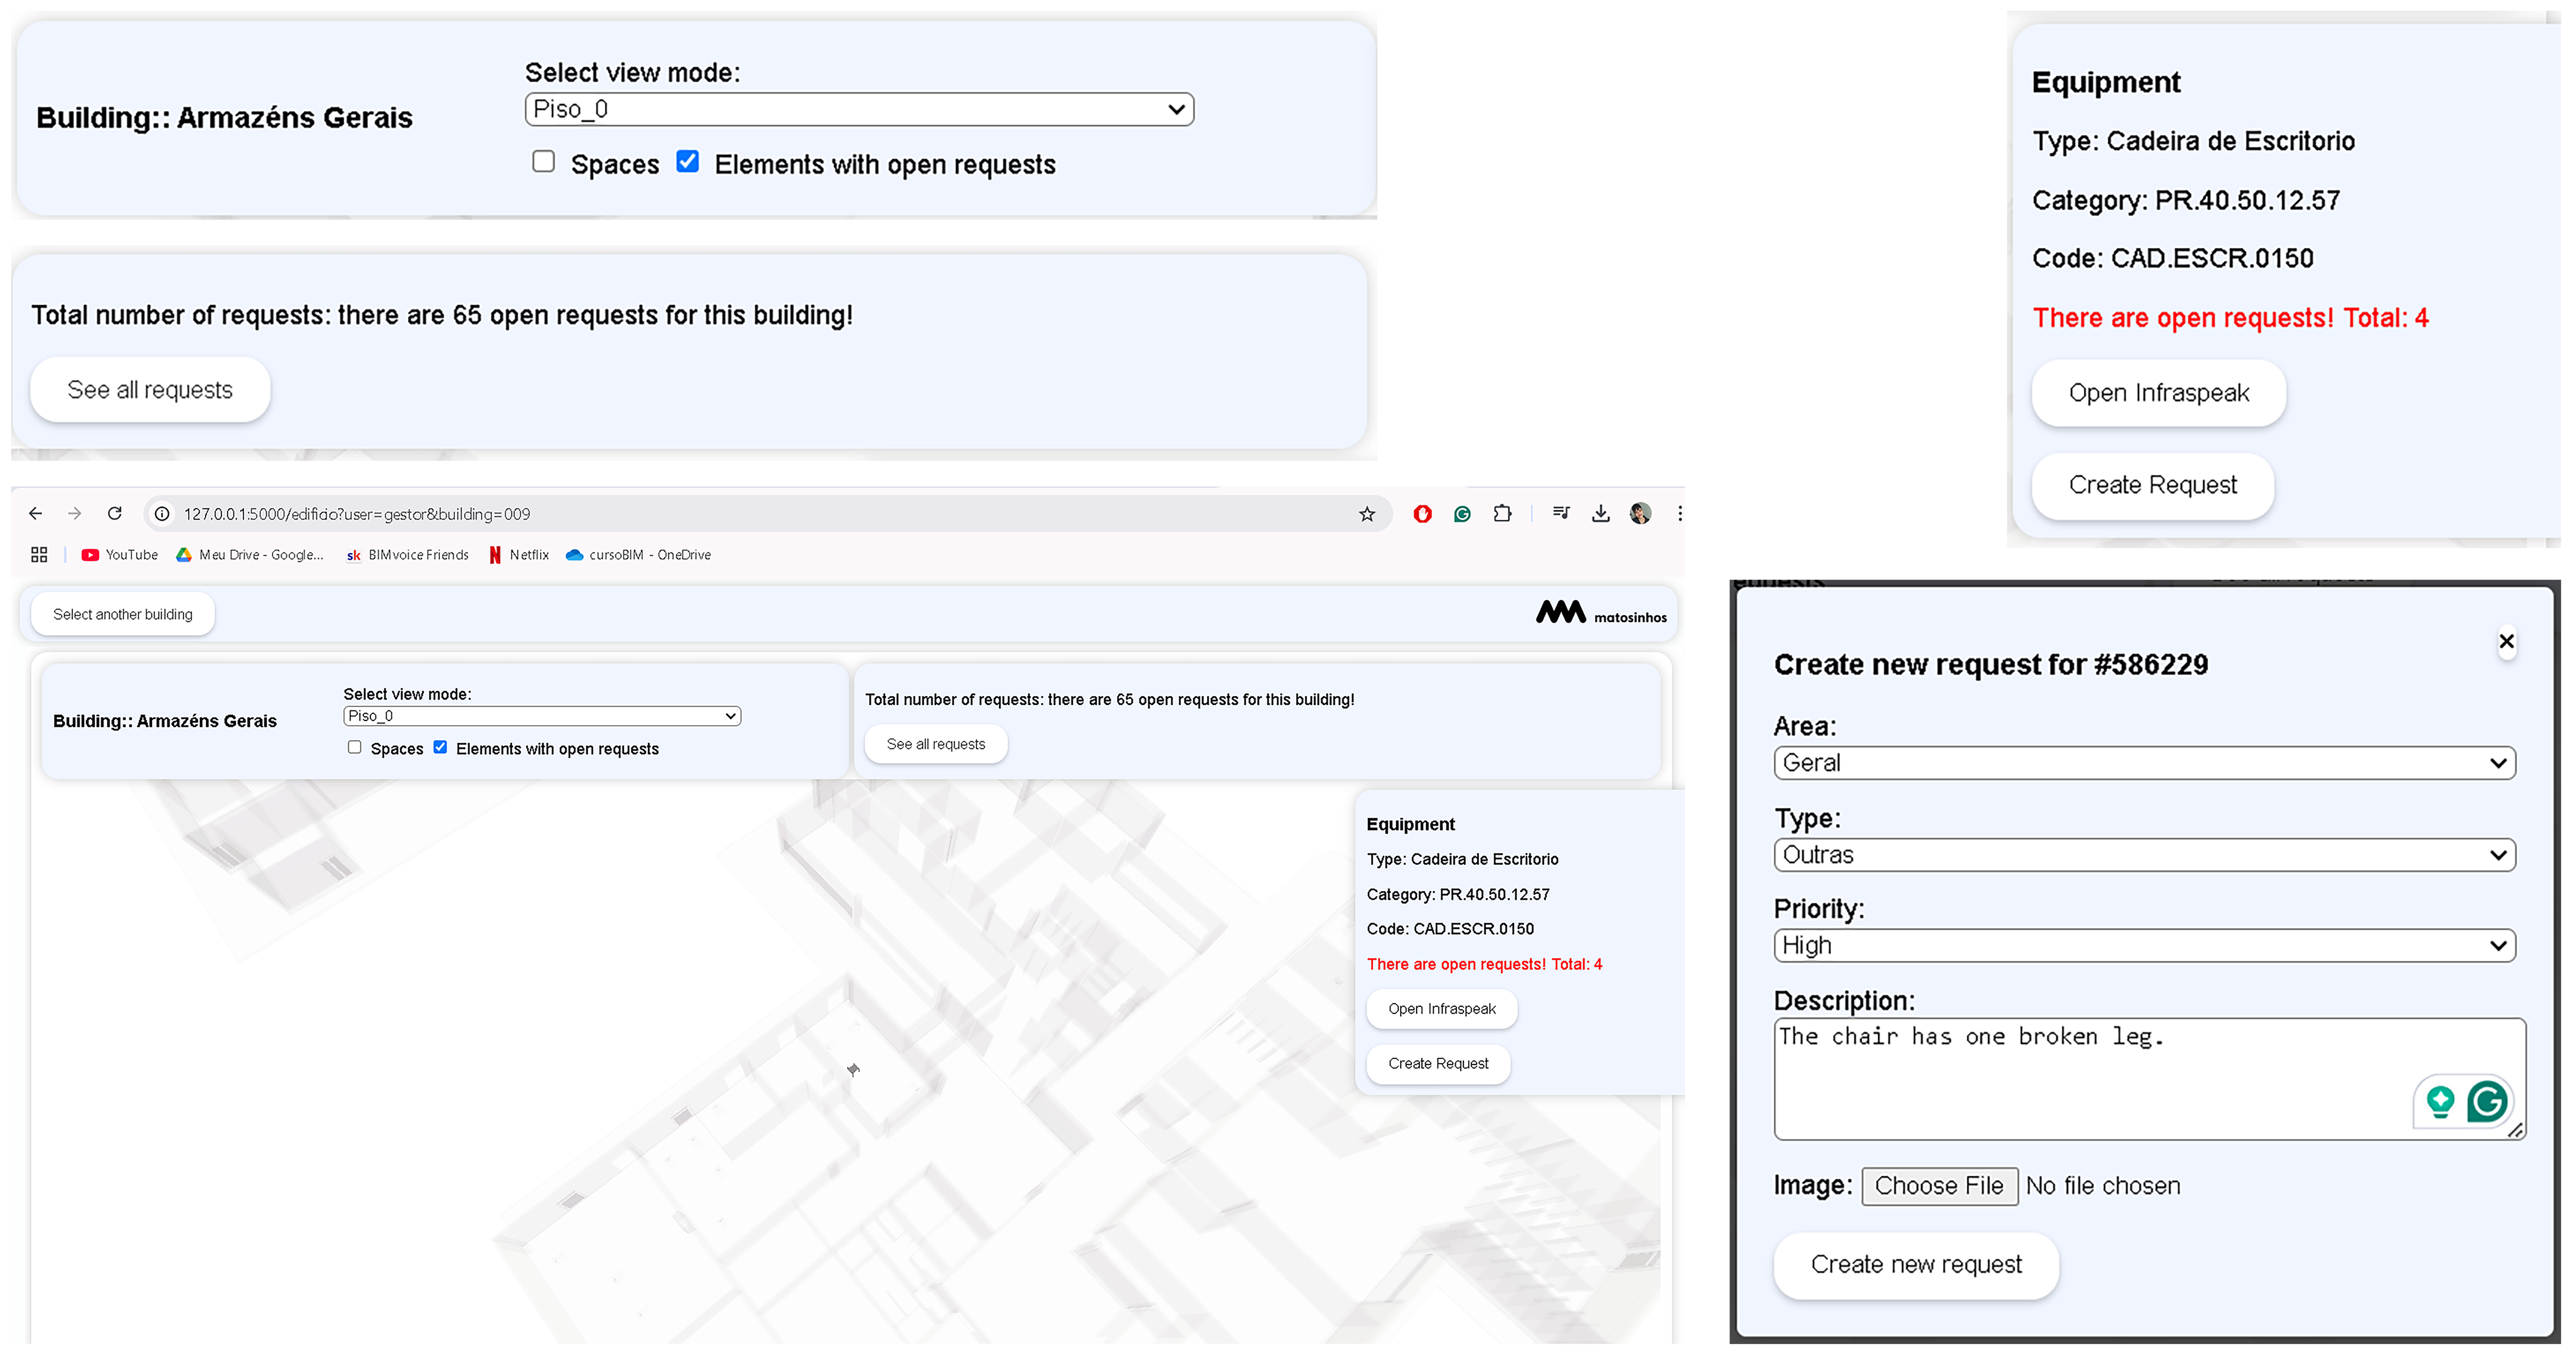
\includegraphics[width=\textwidth]{Images/plataforma_parcial.png}
    \caption{Web platform – visualization mode (a), open building's requests (b) and information about selected element (c)}
    \label{fig_plataforma}
\end{figure*}

\section{Discussion and conclusion}
\label{sec:conclusion}

This work supports the implementation of the BIM methodology in the context of operations management, specifically in the area of integrating the methodology into existing management platforms. Challenges not yet foreseen were encountered during development. In particular, in terms of defining unique identifiers within CMMatosinhos' inventory, the coding used to organise its inventory was not functional for integration with other databases. This was because the existing coding did not uniquely identify a single asset, which meant that elements had to be identified using a combination of two codes (element id and local id). The iterative process used, with periodic meetings with CMMatosinhos, allowed these and other limitations to be overcome. Throughout the process, some optimisations were necessary to improve the user experience when interacting with the platform. For example, the automated mapping between elements and requests had an impact on the final product by reducing the user's waiting time for information to be updated. It should be noted that the IFCjs library and its great capacity for customisation are of great support to the development of web platforms in the context of using the BIM methodology. Through the library, the platform developed can be customised to the end user's objectives. In the context of this work, changes to visualisations (building, floor and elements with open requests) could be implemented, and it was also possible to investigate the model to extract the information needed for the integration platform to work. Finally, the work carried out advances knowledge of the implementation of BIM for building operations by showing a real case in which the methodology can be applied to an existing management system by integrating the information model with a management platform already used by the building manager.

\emph{erro}

operations. The decision-making process presented can be used to implement other integration processes to be developed in the building operations sector.

\section{Acknowledgements}
\label{sec:acknowledgements}

This work was partially funded by FCT/MCTES through national funds (PIDDAC) within the scope of the R\&D unit of the Institute for Sustainability and Innovation in Structural Engineering (ISISE), under reference UIDB/04029/2020 (doi.org/10.54499/UIDB/04029/2020), and within the scope of the ARISE Associated Laboratory for Advanced Production and Intelligent Systems under reference LA/P/0112/2020. This work was also funded by the doctoral scholarship (PRT/BD/154416/2023) awarded to the first author by the Foundation for Science and Technology (FCT), under the MIT Portugal Programme.

\bibliography{ISARC}

\end{document}
